%%%%%%%%%%%%%%%%%%%%%%%%%%%%%%%%%%%%%%%%%
% HW Template
% LaTeX Template
% Version 1.0 (19/10/18)
% Modified by
% Erdem TUNA
% Halil TEMURTAŞ 
% Enes TAŞTAN 
%%%%%%%%%%%%%%%%%%%%%%%%%%%%%%%%%%%%%%%%%
%
%----------------------------------------------------------------------------------------
%	PACKAGES AND OTHER DOCUMENT CONFIGURATIONS
%----------------------------------------------------------------------------------------
\documentclass[a4paper,12pt]{article}
%-----packages------
\usepackage[a4paper, total={6.2in, 8.5in}]{geometry}
\usepackage[english]{babel}
\usepackage[utf8x]{inputenc}
\usepackage{amsmath}
\usepackage{graphicx}
\usepackage[colorinlistoftodos]{todonotes}
\usepackage{gensymb} % this could be problem
\usepackage{float}
\usepackage{fancyref}
\usepackage{subcaption}
\usepackage[toc,page]{appendix} %appendix package
\usepackage{xcolor}
\usepackage{listings}
\usepackage{xspace}
\usepackage{amssymb}
\usepackage{nicefrac}
\usepackage{gensymb}
\usepackage{fancyhdr}
\usepackage{blindtext}  % for dummy text, use \blindtext or \BlindText
\usepackage{lipsum}    % for dummy text, use \lipsum[3-56]
\usepackage[final]{pdfpages}  % pdf include
\usepackage{array} %allows more options in tables
\usepackage{pgfplots,pgf,tikz} %coding plots in latex
\usepackage{capt-of} % allows caption outside the figure environment
\usepackage[export]{adjustbox} %more options for adjusting the ../images
\usepackage{multicol,multirow,slashbox} % allows tables like table1
%\usepackage[hyperfootnotes=false]{hyperref} % clickable references
\usepackage{epstopdf} % useful when matlab is involved
%\usepackage{placeins} % prevents the text after figure to go above figure with \FloatBarrier 
%\usepackage{listingsutf8,mcode} %import .m or any other code file mcode is for matlab highlighting

%-----end of packages

%-----specifications-----
\definecolor{mGreen}{rgb}{0,0.6,0} % for python
\definecolor{mGray}{rgb}{0.5,0.5,0.5}
\definecolor{mPurple}{rgb}{0.58,0,0.82}
\definecolor{mygreen}{RGB}{28,172,0} % color values Red, Green, Blue for matlab
\definecolor{mylilas}{RGB}{170,55,241}

\setcounter{secnumdepth}{5} % how many sectioning levels to assign numbers to
\setcounter{tocdepth}{5}    % how many sectioning levels to show in ToC

\lstdefinestyle{CStyle}{
	commentstyle=\color{mGreen},
	keywordstyle=\color{magenta},
	numberstyle=\tiny\color{mGray},
	stringstyle=\color{mPurple},
	basicstyle=\footnotesize,
	breakatwhitespace=false,         
	breaklines=true,
	frame=single,
	rulecolor=\color{black!40},                 
	captionpos=b,                    
	keepspaces=true,                 
	numbers=left,                    
	numbersep=5pt,                  
	showspaces=false,                
	showstringspaces=false,
	showtabs=false,                  
	tabsize=2,
	language=C
}

\lstset{language=Matlab,%
	%basicstyle=\color{red},
	breaklines=true,%
	frame=single,
	rulecolor=\color{black!40},
	morekeywords={matlab2tikz},
	keywordstyle=\color{blue},%
	morekeywords=[2]{1}, keywordstyle=[2]{\color{black}},
	identifierstyle=\color{black},%
	stringstyle=\color{mylilas},
	commentstyle=\color{mygreen},%
	showstringspaces=false,%without this there will be a symbol in the places where there is a space
	numbers=left,%
	numberstyle={\tiny \color{black}},% size of the numbers
	numbersep=9pt, % this defines how far the numbers are from the text
	emph=[1]{for,end,break},emphstyle=[1]\color{red}, %some words to emphasise
	%emph=[2]{word1,word2}, emphstyle=[2]{style},    
}


\tikzset{
	desicion/.style={
		diamond,
		draw,
		text width=4em,
		text badly centered,
		inner sep=0pt
	},
	block/.style={
		rectangle,
		draw,
		text width=10em,
		text centered,
		rounded corners
	},
	cloud/.style={
		draw,
		ellipse,
		minimum height=2em
	},
	descr/.style={
		fill=white,
		inner sep=2.5pt
	},
	connector/.style={
		-latex,
		font=\scriptsize
	},
	rectangle connector/.style={
		connector,
		to path={(\tikztostart) -- ++(#1,0pt) \tikztonodes |- (\tikztotarget) },
		pos=0.5
	},
	rectangle connector/.default=-2cm,
	straight connector/.style={
		connector,
		to path=--(\tikztotarget) \tikztonodes
	}
}

\tikzset{
	desicion/.style={
		diamond,
		draw,
		text width=4em,
		text badly centered,
		inner sep=0pt
	},
	block/.style={
		rectangle,
		draw,
		text width=10em,
		text centered,
		rounded corners
	},
	cloud/.style={
		draw,
		ellipse,
		minimum height=2em
	},
	descr/.style={
		fill=white,
		inner sep=2.5pt
	},
	connector/.style={
		-latex,
		font=\scriptsize
	},
	rectangle connector/.style={
		connector,
		to path={(\tikztostart) -- ++(#1,0pt) \tikztonodes |- (\tikztotarget) },
		pos=0.5
	},
	rectangle connector/.default=-2cm,
	straight connector/.style={
		connector,
		to path=--(\tikztotarget) \tikztonodes
	}
}
%-----end of specifications-----


%----commands----
\newcommand\nd{\textsuperscript{nd}\xspace}
\newcommand\rd{\textsuperscript{rd}\xspace}
\newcommand\nth{\textsuperscript{th}\xspace} %\th is taken already
\newcommand{\specialcell}[2][c]{ \begin{tabular}[#1]{@{}c@{}}#2\end{tabular}} % for too long table lines

\newcommand{\blankpage}{
	\- \\[9cm]	
	{ \centering \textit{This page intentionally left blank.} \par }
	\- \\[9cm]
}% For Blank Page

\makeatletter
\renewcommand\paragraph{\@startsection{paragraph}{4}{\z@}%
	{-2.5ex\@plus -1ex \@minus -.25ex}%
	{1.25ex \@plus .25ex}%
	{\normalfont\normalsize\bfseries}}
\makeatother
%-----end of commands-----


\pagestyle{fancy}
\fancyhead[LO,LE]{Halil TEMURTAŞ / 2094522   }
\fancyhead[RO,RE]{\today}
\fancyfoot[RO,RE]{
\includegraphics[width=2.7cm]{images/eelogo}}

\begin{document}
\begin{center}
	\textbf{\large EE430 Digital Signal Processing \\[0.2cm] HW 2} \\
\end{center}

\begin{enumerate}
	\item The impulse response of the system is given as $h[n]=\delta [n]-\sqrt{2}\delta [n-1]+\delta [n-2]$	
%		\begin{figure}[H]
%			\center
%			\setlength{\unitlength}{\textwidth} 
%			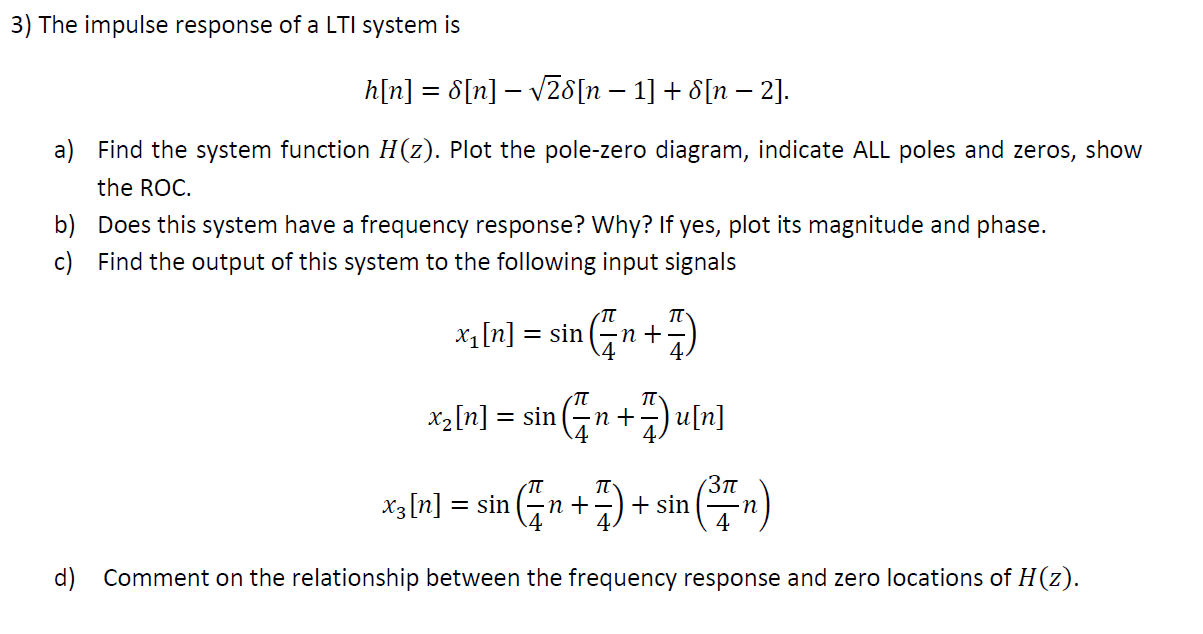
\includegraphics[width=1.0\unitlength]{images/Q3}
%			\caption{\label{fig:Q1}Q1 }
%		\end{figure}
		
		\begin{enumerate} 
			\item The system function $H(z)$ can be found as follows;
				$$	\mathcal{Z} \{	\delta [n]\} = 1 \ \ \forall z	$$
				$$	\mathcal{Z} \{ x[n-n_0] \} = z^{-n_0}X(z)	$$ 
				Thus,
				$$\boxed{	H(z)= 1-\sqrt{2} z^{-1}+z^{-2}	 }$$
			
			$H(z)$ can be put in more classical transfer  function form to find poles and zeros. 
			$$	H(z)= \frac{z^2-\sqrt{2}z + 1}{z^2}=\frac{\left(z-(\frac{1}{2}+\frac{j}{2})\right)\left(z-(\frac{1}{2}-\frac{j}{2})\right)}{z^2}	$$
			Therefore, poles and zeros of the system function can be easily found to be as,
			$$\boxed{ z_{1,2}=\frac{1}{2} \mp \frac{j}{2} } \ , \ \boxed{ p_{1,2}=0 } $$
			Since the impulse response of the system is finite-length , the region of convergence of system function is \textbf{All Z Plane} except $z=0$ due to poles.Pole-zero plot can be seen at \textit{Figure~\ref{fig:Q1b}}.
			
			\begin{figure}[H]
				\center
				\setlength{\unitlength}{\textwidth} 
				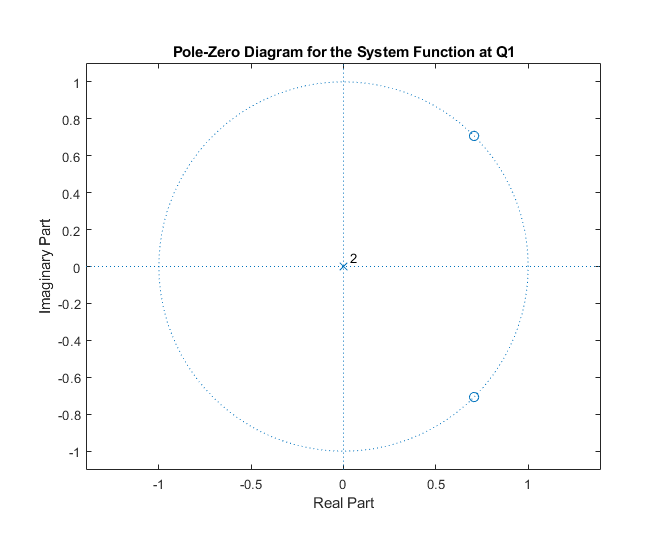
\includegraphics[width=0.675\unitlength]{images/Q1ak}
				\caption{\label{fig:Q1a}Pole-Zero Diagram for the System Function }
			\end{figure}  
 			
 			\item Since the ROC contains the unit circle, the system has a frequency response and it can be found by simply replacing $z$ with $e^{jw}$.
 			
 			$$	H(e^{jw})=H(z)|_{z=e^{jw}} = 1-\sqrt{2} e^{-jw}+e^{-j2w} $$
 			$$ H(e^{jw})=  e^{-jw}[	 e^{jw}+ e^{-jw}-\sqrt{2}]$$
 			$$\boxed {H(e^{jw})= e^{-jw}\left[\cos(w)-\sqrt{2}\right]} $$
 			
 			Magnitude and phase response of the frequency response can be seen at \textit{Figure~\ref{fig:q1b1}} and \textit{Figure~\ref{fig:q1b2}} respectively.
 			
 					
			\begin{figure}[H]
	 			\setlength{\unitlength}{\textwidth} 
 				\centering
				\begin{subfigure}{.5\textwidth}
  					\centering
  					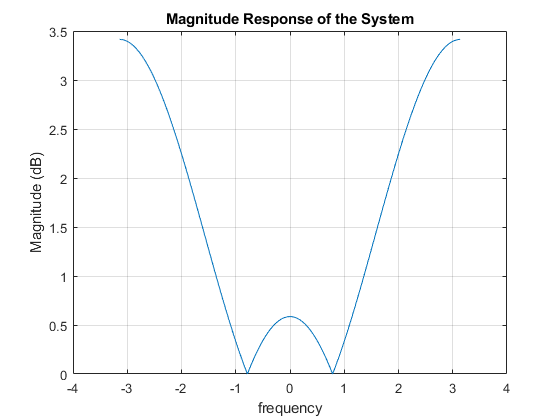
\includegraphics[width=0.48\unitlength]{images/Q1b1k}
  					\caption{\label{fig:q1b1}Magnitude Response }
				\end{subfigure}%
				\begin{subfigure}{.5\textwidth}
  					\centering
					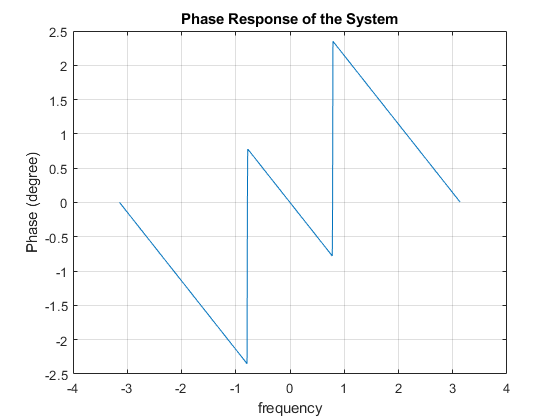
\includegraphics[width=0.48\unitlength]{images/Q1b2k}
  					\caption{\label{fig:q1b2}Phase Response}
				\end{subfigure}
			\caption{\label{fig:Q1b} Magnitude and Phase Response of the System   }
			\end{figure}

 			\item The output of the system for the different inputs can be found using Z-transform of given inputs.
 				\begin{enumerate}
 					\item $	x_1[n]=\sin(\frac{\pi}{4}n+\frac{\pi}{4})=x_1[n]\left(u[-n-1]+u[n]\right)$, since the ROC of the z transform of this input would be empty set, let us use another property of DTFT since we already have frequency response.
 					
 					$$ y[n]=\sum_{k=-\inf}^{\inf}=a_kH(e^{jw})e^{jwn} $$
 					$$	x_1[n]=\sin(\frac{\pi}{4}n)\cos(\frac{\pi}{4})+\sin(\frac{\pi}{4})\cos(\frac{\pi}{4}n)=\frac{1}{\sqrt{2}}\left( \sin(\frac{\pi}{4}n)+\cos(\frac{\pi}{4}n) \right) $$
 					$$	x_1[n]=\frac{1}{\sqrt{2}} \left( \frac{1}{2j}(e^{j\frac{\pi}{4}n-e^{-j\frac{\pi}{4}n}})+\frac{1}{2}(e^{j\frac{\pi}{4}n}+e^{-j\frac{\pi}{4}n}) \right)$$
 					$$	x_1[n]=\frac{1}{2\sqrt{2}}\left( e^{j\frac{\pi}{4}n}(1-j)+  e^{-j\frac{\pi}{4}n}(1+j)	\right)$$
 					Thus,
 					$$ y_1[n]=\frac{1}{2\sqrt{2}}\left( e^{j\frac{\pi}{4}n}(1-j)H(e^{j\frac{\pi}{4}})+  e^{-j\frac{\pi}{4}n}(1+j)H(e^{\frac{-j\pi}{4}})	\right)$$
					Since  $H(e^{j\frac{\pi}{4}})=H(e^{-j\frac{\pi}{4}})=0$
					$$\boxed{ y_1[n]=0 }$$					
 					\item  $x_2[n]=\sin(\frac{\pi}{4}n+\frac{\pi}{4})u[n]$ can be simplifeid further as follows;
 						$$x_2[n]= \frac{1}{\sqrt{2}} \left( \sin(\frac{\pi}{4}n)+\cos(\frac{\pi}{4}n) \right) $$
%%	 					$$ x_2[n]=\frac{1}{2\sqrt{2}}\left( e^{j\frac{\pi}{4}n}(1-j)+  e^{-j\frac{\pi}{4}n}(1+j)	\right)u[n]$$
%%	 					$$ x_2[n]=\frac{1}{4} \left( e^{j\frac{\pi}{4}n}e^{\frac{-3\pi}{4}}+  e^{-j\frac{\pi}{4}n}e^{\frac{\pi}{4}}	\right)u[n] $$
	 					using 
	 					$$ \mathcal{Z} \{u[n]\} = \frac{1}{1-z^{-1}} \ , \ ROC:|z|>|a|	$$
						$$ \mathcal{Z} \{ z_0^nx[n] \}=X(z/z_0) \ , \ ROC:R_x|z_0|$$ 
						$$ \mathcal{Z} \{ \cos(w_0)n	\}u[n]=\frac{1-\cos(w_0)z^{-1}}{1-2\cos(w_0)z^{-1}+z^{-2}} \ , \ |z|>1$$
						$$ \mathcal{Z} \{ \sin(w_0)n	\}u[n]=\frac{\sin(w_0)z^{-1}}{1-2\cos(w_0)z^{-1}+z^{-2}} \ , \ |z|>1 $$		
 						the z-transform $X_2(z)$ can be found as follow;
 						$$ X_2(z)= \frac{1}{\sqrt{2}} \left( \frac{1-\cos(\frac{\pi}{4})z^{-1}}{1-2\cos(\frac{\pi}{4})z^{-1}+z^{-2}}+ \frac{\sin(\frac{\pi}{4})z^{-1}}{1-2\cos(\frac{\pi}{4})z^{-1}+z^{-2}}\right)$$
 						$$ X_2(z)= \frac{1}{\sqrt{2}} \left( \frac{1-\frac{1}{\sqrt{2}}}{1-\sqrt{2}z^{-1}+z^{-2}}+ \frac{\frac{1}{\sqrt{2}}z^{-1}}{1-\sqrt{2} z^{-1}+z^{-2}}\right)$$
	 						$$ X_2(z)=\frac{1}{\sqrt{2}} \left( \frac{1}{1-\sqrt{2}z^{-1}+z^{-2}} \right) $$
	 						$$ Y_2(z)= X_2(z)H(z)=\frac{1}{\sqrt{2}}$$
	 						$$\boxed{ y[n]=\frac{1}{\sqrt{2}} \delta [n] }$$
	 					\item $x_3[n]=\sin(\frac{\pi}{4}n+\frac{\pi}{4})+\sin(\frac{3\pi}{4}n)$
	 					Using linearity property of Z-Transform, we can safely say that the output for the first term is zero, let us find the output for the second term using the eigenfunction property again,
	 					$$	\sin(\frac{3\pi}{4}n)=\frac{1}{2j} \left(e^{j\frac{3\pi}{4}n}-e^{-j\frac{3\pi}{4}n}\right)$$
	 					$$ y_3[n]=\frac{1}{2j} \left(e^{j\frac{3\pi}{4}n}H(e^{j\frac{3\pi}{4}})-e^{-j\frac{3\pi}{4}n}H(e^{-j\frac{3\pi}{4}})\right) $$
	 					$$H(e^{j\frac{3\pi}{4}})=e^{-j\frac{3\pi}{4}}\left[\cos(\frac{3\pi}{4})-\sqrt{2}\right]=2\sqrt{2}e^{j\frac{\pi}{4}}$$
	 					$$H(e^{-j\frac{3\pi}{4}})=e^{j\frac{3\pi}{4}}\left[\cos(\frac{3\pi}{4})-\sqrt{2}\right]=2\sqrt{2}e^{-j\frac{\pi}{4}}$$
	 					$$ y_3[n]=\frac{2\sqrt{2}}{2j} \left(e^{j(\frac{3\pi}{4}n+\frac{\pi}{4})}-e^{-j(\frac{3\pi}{4}n+\frac{\pi}{4})}\right) $$
	 					$$\boxed{ y_3[n]=2\sqrt{2} \sin(\frac{3\pi}{4}n+\frac{\pi}{4})} $$
	 						 
 				\end{enumerate}
			\item Since on the unit circle, the Z-Transform is equivalent to the DTFT, the zeros of the Z-Transform at unit circle is also the zeros of the DTFT.
		\end{enumerate}
		 
		
			
	\item The system function is given as $H(z)=\frac{1-\sqrt{2}z^{-1}+z^{-2}}{1-2z^{-1}}$
		
		\begin{enumerate}
			\item a
			\item b
			\item 
				$$ H(z)=\frac{Y(z)}{X(z)}=\frac{1-\sqrt{2}z^{-1}+z^{-2}}{1-2z^{-1}}$$
				Thus,
				$$\boxed{ y[n]-2y[n-1]=x[n]-\sqrt{2}x[n-1]+x[n-2] }$$
		\end{enumerate}
				
	\item Since $x[n]$ is a right-sided sequence, the ROC of the  $H(z)$ would be outward. It is implied that the ROC of the $H(z) $ includes $|z|=4$ circle. This means that the ROC can be something close to a ROC at \textit{Figure~\ref{fig:Q3}}. The circle can be smaller but can not be larger that $|z|=4$ since it is given that the Z Transform exist for that circle. 
	
		Thus, in any circumstances, $X(z)$ exists for $z=4.1e^{jw}$ since the ROC includes $|z|=4.1$ circle in any case. However, it is possible that  $X(z)$ may not exist for $z=3.9e^{jw}$ since the ROC may not include $|z|=3.9$ circle as in \textit{Figure~\ref{fig:Q3}}.
	
		\begin{figure}[H]
			\center
			\setlength{\unitlength}{\textwidth} 
			\includegraphics[width=0.675\unitlength]{images/Q3k}
			\caption{\label{fig:Q3}Possible ROC for the Given System}
		\end{figure}
		
		
	
		
	\item Given that $x[n]=\delta [n+1] +{(\frac{1}{2})}^n u[n]$
		
		\begin{enumerate}
			\item $$\boxed{	X(z)=z-\frac{1}{1-\frac{1}{2}z^{-1}}=\frac{z(z+\frac{1}{2})}{z-\frac{1}{2}} \ , \ |z|>\frac{1}{2}	}$$
			$$ \boxed{ p_{a-1}=\frac{1}{2}} \ ,\ \boxed{ p_{a-2}=\inf} \ ,\  \boxed{z_{a-1}=0} \ ,\ \boxed{z_{a-2}=\frac{-1}{2}}  $$
			\item $$\boxed{ \mathcal{Z} \{x[n-5] \} = z^{-5}X(z)=\frac{z+\frac{1}{2}}{z^4(z-\frac{1}{2})} \ , \ |z|>\frac{1}{2}  }$$	
			$$ \boxed{ p_{b-1}=\frac{1}{2}} \ ,\ \boxed{p_{b-2,3,4,5}=0} \ ,\ \boxed{z_{b-1}=\frac{-1}{2}} \ ,\ \boxed{z_{b-2,3,4,5}=\inf} $$
			\item $$ \mathcal{Z} \{nx[n] \} =-z\frac{d}{dz}X(z)=	-z\frac{d}{dz}(\frac{z+\frac{1}{2}}{z^4(z-\frac{1}{2})}) \ , \ |z|>\frac{1}{2} $$
				$$  \mathcal{Z} \{nx[n] \} = -z\left( -\frac{1+z^2}{z^5{(z-0.5}^2)}\right)$$
				$$ \boxed{	\mathcal{Z} \{nx[n] \} = \frac{1+z^2}{z^4{(z-0.5}^2)}}$$
				$$ \boxed{ p_{c-1,2}=\frac{1}{2}} \ ,\ \boxed{ p_{c-3,4,5,6}=0} \ ,\ \boxed{ z_{c-1,2}=\mp j} \ ,\ \boxed{ p_{c-3,4,5,6}=\inf} $$
			\item $$ \cos(\frac{\pi}{2}n)x[n] = \frac{1}{2} \left( e^{j\frac{\pi}{2}n}x[n]+e^{-j\frac{\pi}{2}n}x[n]	\right) $$
			$$ \mathcal{Z} \{\cos(\frac{\pi}{2}n)x[n]\}= \frac{1}{2} \left( X(\cfrac{z}{e^{j\frac{\pi}{2}}}) + X(\cfrac{z}{e^{-j\frac{\pi}{2}}})  \right) $$
			$$\boxed{ \mathcal{Z} \{ \cos(\frac{\pi}{2}n)x[n]\}=\frac{1}{2}\left( 
			\frac{(\cfrac{z}{e^{j\frac{\pi}{2}}})(\cfrac{z}{e^{j\frac{\pi}{2}}}+\frac{1}{2})}{\cfrac{z}{e^{j\frac{\pi}{2}}}-\frac{1}{2}}  +  \frac{(\cfrac{z}{e^{-j\frac{\pi}{2}}})(\cfrac{z}{e^{-j\frac{\pi}{2}}}+\frac{1}{2})}{\cfrac{z}{e^{-j\frac{\pi}{2}}}-\frac{1}{2}}
			\right) }$$
			
		\end{enumerate}
		
	\item $H(z)$ will be in the form of 
		$$\frac{\alpha (z+\frac{1}{2})}{(z-3)(z-\frac{1}{2})} $$
		$$ H(1)=\frac{\alpha (3/2)}{(-2)(1/2)}=1$$
		$$ \boxed{	\alpha=\frac{-2}{3}	}$$
		$$\boxed{ H(z)=-\frac{2}{3}\frac{ (z+\frac{1}{2})}{(z-3)(z-\frac{1}{2})} }$$
		
		\begin{enumerate}
			\item System to be stable, the ROC must include unit circle. The ROC can not also include any pole and should be one piece. Thus the ROC can only be
			$$\boxed{ ROC: \frac{1}{2}<|z|<3 }$$	
			The pole-zero diagram for this system and its ROC can be seen at \textit{Figure~\ref{fig:Q5a}}.
			\begin{figure}[H]
				\center
				\setlength{\unitlength}{\textwidth} 
				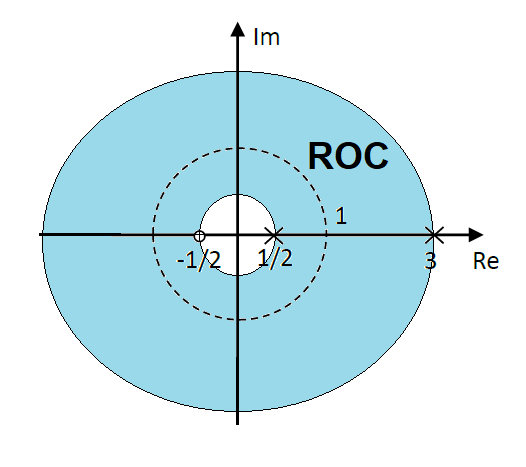
\includegraphics[width=0.675\unitlength]{images/Q5ak}
				\caption{\label{fig:Q5a} ROC for the Given System}
			\end{figure}	
			
			To find $h[n]$, partial fraction method can be used;	
			$$ H(z)=\left[\frac{ a}{z-3}+\frac{b}{z-\frac{1}{2}}\right] $$
			where a and b can be found easily as
			$$ \boxed{a=-\frac{14}{15}} \ , \ \boxed{b=\frac{4}{15}}$$
			Thus, considering the ROC, $h[n]$ becomes;
			$$\boxed{ h[n]= \frac{4}{5}{(\frac{1}{2})}^n u[n]-\frac{14}{15}{(3)}^n u[-n-1] }$$
			\item Given that,
				$$ h_2[n]=h[-n+2] $$
				Z-Transform of $h_2[n]$ can be calculated as follows,
				$$ H_2(z)=z^2X(1/z)=H(z)=-\frac{2}{3}\frac{ z^2(z^{-1}+\frac{1}{2})}{(z^{-1}-3)(z^{-1}-\frac{1}{2})}$$
				
				$$\boxed{H_2(z)=-\frac{2}{9}\frac{ z^3(z+2)}{(z-\frac{1}{3})(z-2)} \ , \ \frac{1}{3}<|z|<2	}$$
				
				Pole-zero diagram for this transform and its ROC can be seen at \textit{Figure~\ref{fig:Q5b}}.
				\begin{figure}[H]
					\center
					\setlength{\unitlength}{\textwidth} 
					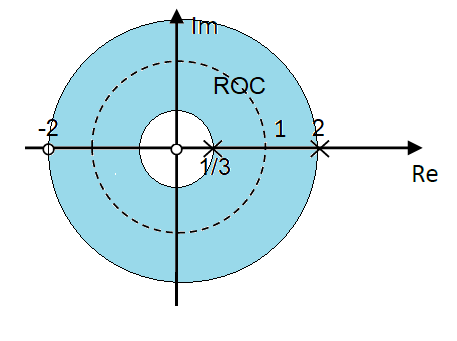
\includegraphics[width=0.675\unitlength]{images/Q5bk}
					\caption{\label{fig:Q5b} ROC for the Updated System}
				\end{figure}
		\end{enumerate}
		
	
	\item Given that
		$$ H(z)=\frac{1-z^{-1}}{1-0.25z^{-2}}=\frac{1-z^{-1}}{(1-0.5z^{-1})(1+0.5z^{-1})}$$
	 
		
		\begin{enumerate}
			\item $$ X(z)=\frac{1}{1-z^{-1}} $$
				$$ Y_1(z)=X_1(z)H(z)=\frac{1}{(1-0.5z^{-1})(1+0.5z^{-1})}=\frac{a}{1-0.5z^{-1}}+\frac{b}{1+0.5z^{-1}}$$
				$$\boxed{a=b=\frac{1}{2}	}$$
				$$ Y_1(z)=\frac{1}{2}(\frac{1}{1-0.5z^{-1}})+\frac{1}{2}(\frac{1}{1+0.5z^{-1}})$$
				
				$$\boxed{	y_1[n]=\frac{1}{2}\left[	{(-0.5)}^n+{(0.5)}^n \right] u[n]}$$
			\item $$Y_2(z)=1-z^{-1}=X_2(z)H(z)$$
				$$X_2(z)=1-0.25z^{-2} $$
				
				$$\boxed{	x_2[n]=\delta [n]-0.25\delta [n-2]	}$$
			\item Since the system is casual
				$$h[n]=0 \ for \ n<0$$
				Thus, the input can behave as $cos(0.5\pi n)u[n]=x_3[n]$.
				$$X_3(z)=\frac{1-\cos(0.5\pi)z^{-1}}{1-2\cos(0.5\pi)z^{-1}+z^{-2}}\ ,\ |z|>1$$
				$$ X_3(z)=\frac{1}{1+z^{-2}} $$
				$$ Y_3(z)=X_3(z)H(z)=	\frac{1-z^{-1}}{(1+z^{-2})(1-0.25z^{-2})}	$$
				
				$$ \boxed{	y_3[n]=\mathcal{Z}^{-1}\{ Y_3(z) \}	}$$		
		\end{enumerate}
	
		
	\item Given that
		$$ \hat{X}(z)=logX(z)$$
		and 
		$$ x[n]=\delta [n]+a\delta [n-N]$$
		$\hat{x}[n]$ can be found as follows,
		$$ X(z)=1+az^{-N} $$
		$$ \hat{X}(z)=\mathcal{log}\{ 1+az^{-N} \} $$
		Using Taylor Series Expansion, more specifically Mercator Series expansion,
		$$	log(1+x)=\sum_{n=1}^{\inf}({-1})^{n+1}\frac{x^n}{n}=x-\frac{x^2}{2}+\frac{x^3}{3}.....	$$
		assume, $x=az^{-N}$ for our case,
		$$ \hat{X}(z)=\sum_{n=1}^{\inf}({-1})^{n+1}\frac{az^{-Nn}}{n} $$
		Thus,
		$$\boxed{ \hat{x}[n]=\sum_{n=1}^{\inf} \frac{({-1})^{n+1}}{n}\delta[n-Nn] }$$
		
	\item Given that
		$$ c_{xx}[n]=\sum_{k=-\inf}^{\inf} x[k]x[k+1] $$
		
		\begin{enumerate}
			\item $$ C_{xx}(z)=\sum_{n=-\inf}^{\inf} \sum_{k=-\inf}^{\inf} x[k]x[k+n]z^{-n} $$
				$$ C_{xx}(z)=\sum_{k=-\inf}^{\inf} x[k] \sum_{n=-\inf}^{\inf} x[k+n] z^{-n}$$
				Let $m=k+n$
				$$ C_{xx}(z)=\sum_{k=-\inf}^{\inf} x[k]z^k \sum_{m=-\inf}^{\inf} x[m] z^{-m}$$
				$$ C_{xx}(z)=\sum_{k=-\inf}^{\inf} x[k]z^k X(z)$$
				Let $\hat{k}=-k$
				$$ C_{xx}(z)=\sum_{\hat{k}=-\inf}^{\inf} x[-\hat{k}]z^{-\hat{k}} X(z)$$
				$$ C_{xx}(z)=\mathcal{Z}\{x[-k]\} X(z)$$
				
				$$\boxed{ C_{xx}(z)=X(\frac{1}{z}) X(z) }$$
				
				
			\item 
				$$X(z)=\frac{1}{1-az^{-1}} $$
				$$X(z^{-1})=\frac{1}{1-az} $$
				$$ C_{xx}=X(z)X(z^{-1})=\frac{1}{(1-az^{-1})(1-az)}=\frac{-az^{-1}}{(1-az^{-1})(1-a^{-1}z^{-1})} $$
				$$ C_{xx}=\frac{a_1}{1-az^{-1}}+\frac{a_2}{1-a^{-1}z^{-1}}$$
				$$ \boxed{a_1=-\frac{1}{1-a^{-2}}} \ , \  \boxed{a_2=-\frac{a^2}{1-a^2}} $$
Since it is stable, the ROC includes unit circle. Thus, ROC would be in a ring form. Assuming $a<1$ and $1/a>1$, the ROC becomes $\frac{1}{a}<|z|<a$. Considering the ROC, $c_{xx}$ becomes,
				
				$$ \boxed{c_{xx}[n]=-\frac{1}{1-a^{-2}}a^nu[n]--\frac{a^2}{1-a^2}a^{-n}u[-n-1] }$$
				The pole-zero diagram and ROC foe the given system can be seen at \textit{Figure~\ref{fig:Q8b}}.
				\begin{figure}[H]
					\center
					\setlength{\unitlength}{\textwidth} 
					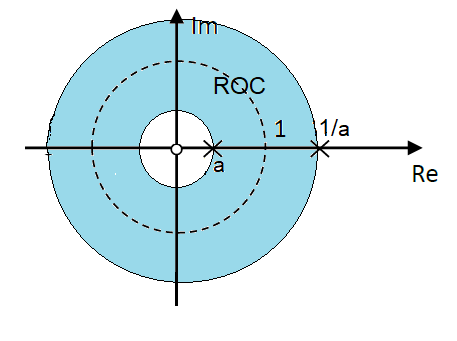
\includegraphics[width=0.675\unitlength]{images/Q8bk}
					\caption{\label{fig:Q8b} ROC for Given System}
				\end{figure}
			\item It is clear that $c_{xx}(z)=c_{xx}(z^{-1})$. Thus, $x[-n]$ would have same autocorrelation function with $x[n]$.
			\item Also notice that $ C_{xx}=X(z)X(z^{-1})=\frac{1}{(1-az^{-1})(1-az)} $, if we could have only extra polynomial at the dominator like $z^{-l}$, we could potentially get rid of it as we multiply with $z^l$ term of $X(z^{-1})$. This can be satisfied with any shifted version of $x[n]$, i.e., $x[n-l]$
		\end{enumerate}
	
	\item 9th Question
		
		\begin{enumerate}
			\item Z-Transfer found using conv command can be seen at \textit{Figure~\ref{fig:Q9a}}. The source code for this part can be found in \textbf{Appendix B}.
				\begin{figure}[H]
					\center
					\setlength{\unitlength}{\textwidth} 
					\includegraphics[width=1.0\unitlength]{images/Q9ak}
					\caption{\label{fig:Q9a} Z-Transfer using conv command}
				\end{figure}
			\item Inverse Z-Transform of the given system function using residuez can be seen at \textit{Figure~\ref{fig:Q9b2}}. The source code for this part can be found in \textbf{Appendix B}.
				
				
				\begin{figure}[H]
					\center
					\setlength{\unitlength}{\textwidth} 
					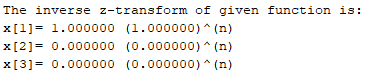
\includegraphics[width=0.8\unitlength]{images/Q9b2k}
					\caption{\label{fig:Q9b2} Inverse Z-Transform of the Given System Function}
				\end{figure}
				
			\item Pole-Zero diagram for the system function given can be seen at \textit{Figure~\ref{fig:Q9c}}. The source code for this part can be found in \textbf{Appendix B}.
				\begin{figure}[H]
					\center
					\setlength{\unitlength}{\textwidth} 
					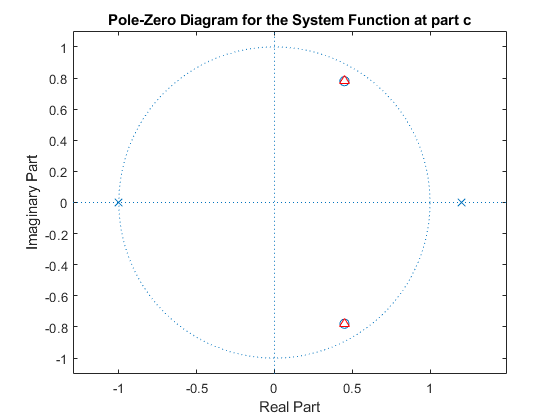
\includegraphics[width=1.0\unitlength]{images/Q9ck}
					\caption{\label{fig:Q9c} Pole-Zero Diagram for the System Function Given at part c}
				\end{figure}
		\end{enumerate}
\end{enumerate}
	\newpage
\begin{appendices}
	\section{Source Code for Question 1}
%%	\lstinputlisting[language=Matlab,firstline=33, lastline=34]{q13.m} \-\\[1cm]		
		\lstinputlisting[language=Matlab]{Q1.m} 
		\newpage
	\section{Source Code for Question 9}
		\lstinputlisting[language=Matlab]{Q9.m} 
\end{appendices}
\end{document}

%----samples------
%\begin{itemize}
%\item Item
%\item Item
%\end{itemize}

%\begin{figure}[H]
%\center
%\setlength{\unitlength}{\textwidth} 
%\includegraphics[width=1.0\unitlength]{../images/logo1}
%\caption{\label{fig:logo}Logo }
%\end{figure}

%\begin{figure}[H]
%	\setlength{\unitlength}{\textwidth} 
%	\centering
%	\begin{subfigure}{.5\textwidth}
%  		\centering
%  		\includegraphics[width=0.48\unitlength]{../images/logo1}
%  		\caption{\label{fig:logo1}Logo1 }
%	\end{subfigure}%
%	\begin{subfigure}{.5\textwidth}
%  		\centering
%		\includegraphics[width=0.48\unitlength]{../images/logo2}
%  		\caption{\label{fig:logo2}Logo2}
%	\end{subfigure}
%\caption{\label{fig:calisandegree} Small Logos   }
%\end{figure}
	
%\begin{table}[H]
%  \centering
% 
%    \begin{tabular}{c|c|c}
%       $$A$$ & $$B$$ & $$C$$ \\ \hline
%       1 & 2 & 3  \\ \hline
%       2 & 3 & 4  \\ \hline
%       3 & 4 & 5  \\ \hline
%       4 & 5 & 6  
%      
%  \end{tabular}
%  \caption{table}
%  \label{tab:table}
%\end{table}
	
%\begin{table}[H]
%  \centering
% 
%    \begin{tabular}{c|c|c}
%       \backslashbox{$A$}{$a$} & $$\specialcell{ Average deviation \\ after subtracting out the  \\ frequency error }$$ & $$C$$ \\ \hline
%       \multirow{2}{*}{1} & 2 & 3  \\ \cline{2-3}
%        & 3 & 4  \\ \hline
%       3 & \multicolumn{2}{c}{4}  \\ \hline
%       4 & 5 & 6  
%      
%  \end{tabular}
%  \caption{table}
%  \label{tab:table}
%\end{table}
%-----end of samples-----